\documentclass{article}
\usepackage[margin=2cm]{geometry}
\usepackage{graphicx}
\graphicspath{ {c:/images/} }
\title{NavUP: Architectural Requirements Specifications and Design}
\author{	 
	Greeff, Claude\\
	\texttt{u13153740@tuks.co.za}
	\and	
}
\begin{document}
	\maketitle
	\section{Architecture Requirements}
		\subsection{Quality Requirements}
		 To create a safe working system that will meet all the required specifications of the NavUP project, specific system requirements need to be looked at in depth. The following are the system requirements that need to be considered. Security, reliability, efficiency, maintainability and usability.
		 
		 \subsubsection{Security}
		 Security is concerned with unauthorized access to specific software functions. An important security measure that needs to be satisfied by the NavUP system is the confidentiality of different user level usernames and passwords. Personal usernames will be set by each user, or their student/staff number will be used to log in. Each user will be required to set their own password. Passwords will be required to be more than 7 characters in length to decrease the likely hood of potential hackers hacking passwords successfully. In the case of a forgotten password, a users password may be reset via a link and an email with a One Time Password. If a user has entered the incorrect password more than 3 times, the account should be blocked and the user should be notified for a password reset. Passwords and any related personal information will be encrypted and safely stored in a 'Users' database.
		 
		  Specific locations will be linked to each user profile. Security will be put in place to allow only that user or other users whom the location is shared with to see the pinned location. Access to the NavUP system will only be made available through the University of Pretoria's firewall network. The firewall will hold as a barrier to deny any outside activity. As different levels of user exist each user will have a specific degree of authority. Admin users will be able to add and remove locations, venues and more permanent locations that will effect the map of the NavUP database. Admin users will have the power to remove lower priority users unwanted actions.
		 
		\subsection{Reliability}
		Concerned with the level of risk and chance of application failure. To increase reliability, downtime needs to be reduced and prevented as well as application errors affecting users. Users will need to be navigated to specific locations for classes, practicals and crucial meetings. User authority needs to be kept in place, not allowing users access to prohibited functions allowing them to make unwanted changes to the NavUP system. The NavUP system will need the ability to recover from a failed state, bring back the system to full operation. Finally the NavUP application should withstand any environmental threats that have the potential to cause system failure.
		 
		\subsection{Efficiency}
		The two primary sub characteristics of efficiency are broken down into, time behavior and resource behavior. The performance of the NavUP application will be a reflection of how efficient the resources have been used within the application. This will have an effect on the battery life of mobile devices as they are engineered to have a longer life with less processing being done.
		By making use of a microservice architecture we will develop a suite of independent and deployable software services, structuring each non-functional requirement into logical, coherent modules, utilizing the correct design patterns and designs, resulting in maximum efficiency.
		
		\subsection{Maintainability}
		As previously mention, each non-functional requirement will be structured logically, enabling future programmers to understand and make necessary changes without the headache of trying to figure out what each code service's purpose is. Due to each software service being independent it will allow code to be worked on without total service down time, this too will contribute to the overall stability, testability and analyzability in identifying the root cause of a failure within the application software.
		
		\subsection{Usability}
		The usability is of utmost importance, as we will have a variety of users making use of the NavUP application. Users will range from individuals who are experts at using mobile devices to older generation users who might not be as experienced in using mobiles devices and applications. Features and functions will be easy to understand and use maximizing user experience and making it easy for new users to learn how the application functions.		
	
	\section{Architecture Constraints}
	Constraints are a result of design decisions that are fixed and may not be altered. Constraints may be intentional or unintentional often provided by stakeholders committed toward the project.
		
		\subsection{Programming Language Constraints}
			\begin{itemize}
 				\item Web Based Development
 				\bigskip
 				\\ 				
 				The web based development will make use of a variety of programming languages. HTML, CSS, JavaScript and JSON will be the minimum required languages needed to deliver what is expected.
 				
 				All the client validation will be done using JavaScript, checking user input validation.			
 				
  				\item Server Side Development
  				\bigskip
 				\\
 				User information, information regarding locations and venues will be stored within a database. To run the database we will make use of mySQL and PHP and AJAX, where validation will be done by PHP.
 				
 				\item Mobile Application  Development
  				\bigskip
 				\\
 				The mobile application will be built using Android Studio (Java).
 							
			\end{itemize}
			
		\subsection{Operating System Constraints}			   
 				The NavUP application needs to run on Windows, iOS and Android at the very least. Building software that fails to satisfy the platform constraint means we have failed to deliver what is expected by the external stakeholder. 
 				
 		\subsection{Network Constraints}			 
 				The NavUP application will run on the Universities network allowing only users within the firewall to make use of the application.
 				
 	\pagebreak
 	
 	\section{Architectural Patterns or Styles}
 	We will be implementing the microservices architectural pattern. As well as different architectural patterns for each subsystem
 	
 		\subsection{Benefits}
 			\begin{itemize}
 				\item Deployability
 				\bigskip
 				\\
 				Redeployment is not necessary when changes are made to code preventing the risk of disruption.
 				Developers are able to deploy independent services without having to wait on others to complete their modules, this improves time management and contributes to the overall flexibility.
 				\item Changeability
 				\bigskip
 				\\
 				Due to constant changes in technologies and user requirements upgrades need to be made to adapt to these new changes. Microservices  facilitate this very well allowing independent services to be upgraded.
 				\item Ability to Utilize Different Technologies
 				\bigskip
 				\\
 				Java may be used for event processing microservices due to multithreading properties of JVM.
 				This allows programmers to make use of new technologies on services without disrupting of causing system failure.
 				\item System Resilience
 				\bigskip
 				\\
 				If a microservice stops working, only small, very specific functionality will be lost. This enables programmers to build resilience by making use of smaller independent services.
 			\end{itemize}
 		\subsection{Concerns}
 			\begin{itemize}
 				\item Complexity
 				\bigskip
 				\\
 			\end{itemize}
 			 \subsection{Architectural Patterns for subsystems}
				\subsection{User Subsystem}
				For the User module we will be using a layered architecture, allowing the use of dependency injection allowing for pluggable application architectures
					\subsection{Benefits}
 						\begin{itemize}
 							\item Seperation of Concerns
 							\bigskip
 							\\
 							Seperates the business logic from the presentation, thus allowing you to work on seperate layers independently, allowing non-repeatability
 							\item Flexibility
 							\bigskip
 							\\
 							Coping with growth or traffic will be easier to handle.
 							\item Each layer can evolve independently
 							\bigskip
 							\\
 							Since each layer is independent from each other, each layer will be able to change without affecting any of the other layers.
 							\item proven and stable protocols and design
 							\bigskip
 							\\
 							 One of the most commonly used architectures means that protocols and designs means the system will be stable.
 						\end{itemize} 
	\subsection{Concerns}
 			
 				There are many problems that can occur but the main one would be how to design the application so that it supports maintainability, extensibility, security and scalability.
			
	\subsection{Design of the Architecture}
		\begin{itemize}
 				\item Class Diagram
				
 			
				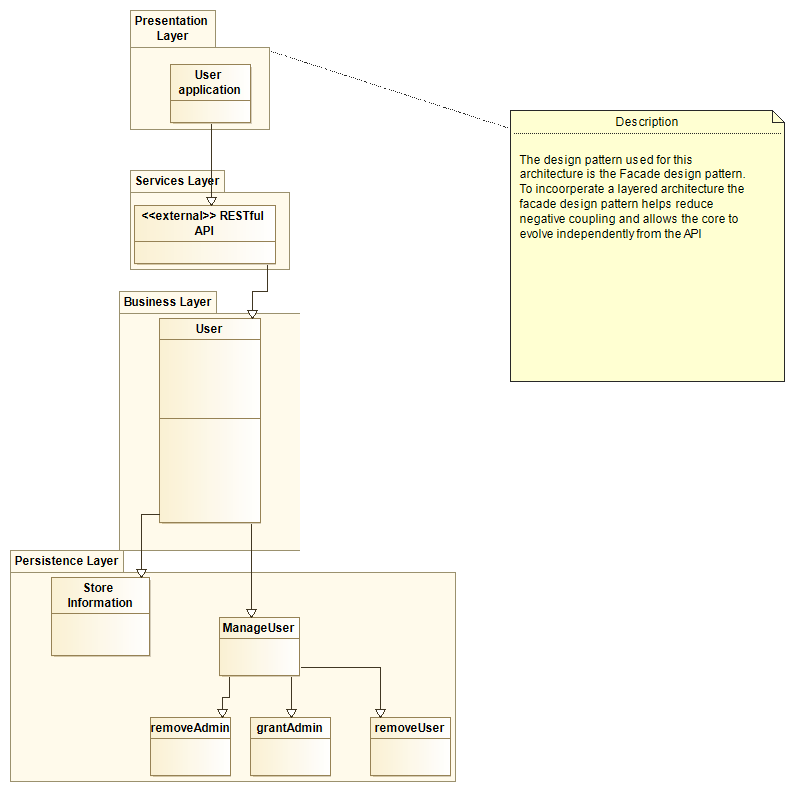
\includegraphics[scale=0.75]{cdu.png}
 				\\
				\\
				\\
				\\
				\item Sequence Diagram
				
 				
				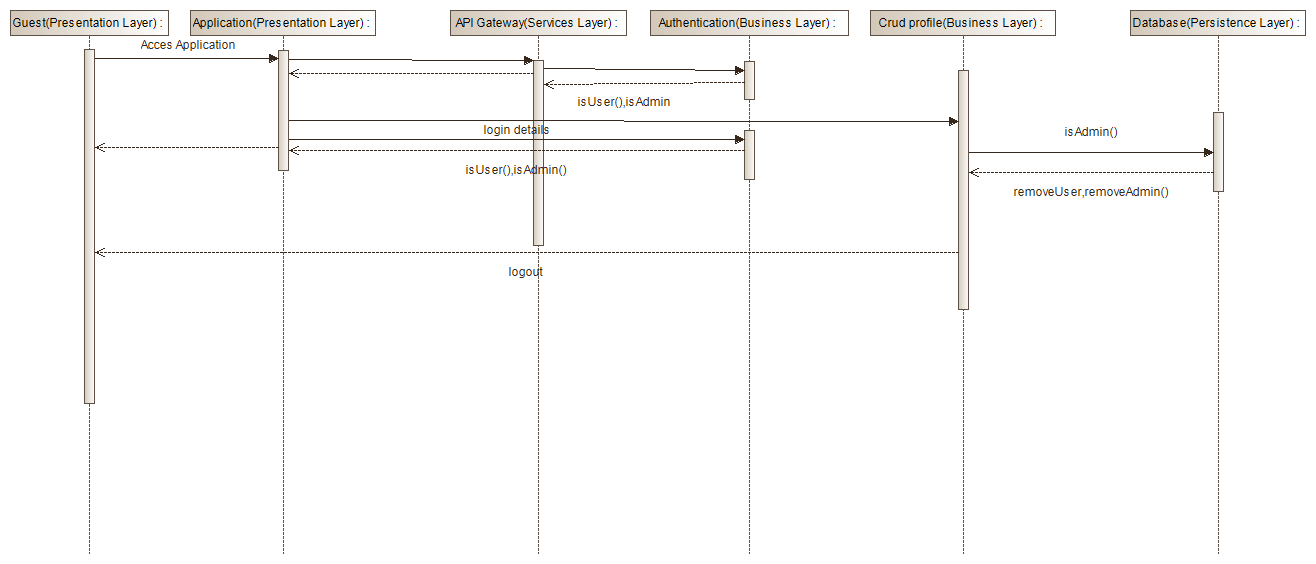
\includegraphics[scale=0.4]{isdu.png}
				\\
				\\
				\\
				\\
				\item Use Case Diagram

	
				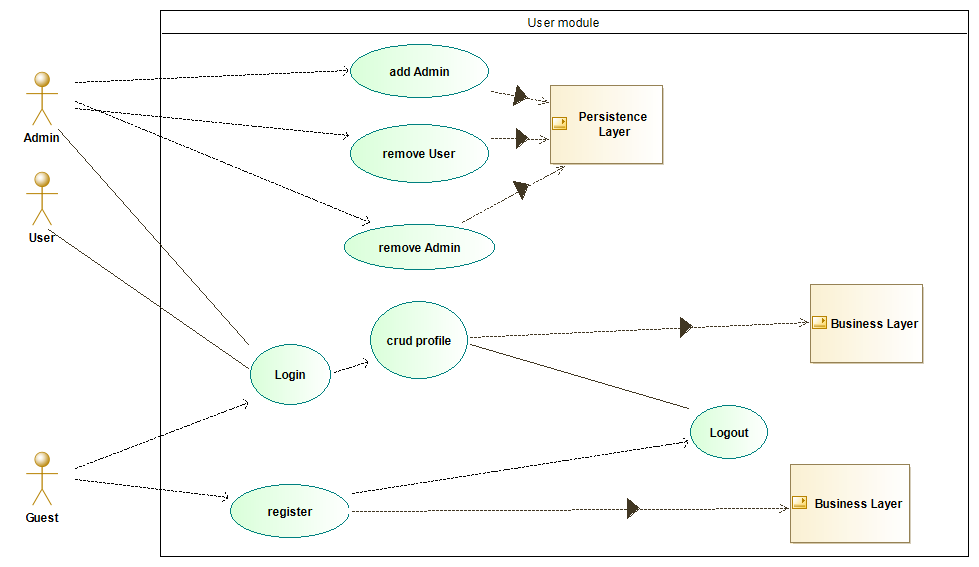
\includegraphics[scale=0.75]{uuc.png}
				\\
				\\
				\\
				\\
				\item State Diagram
				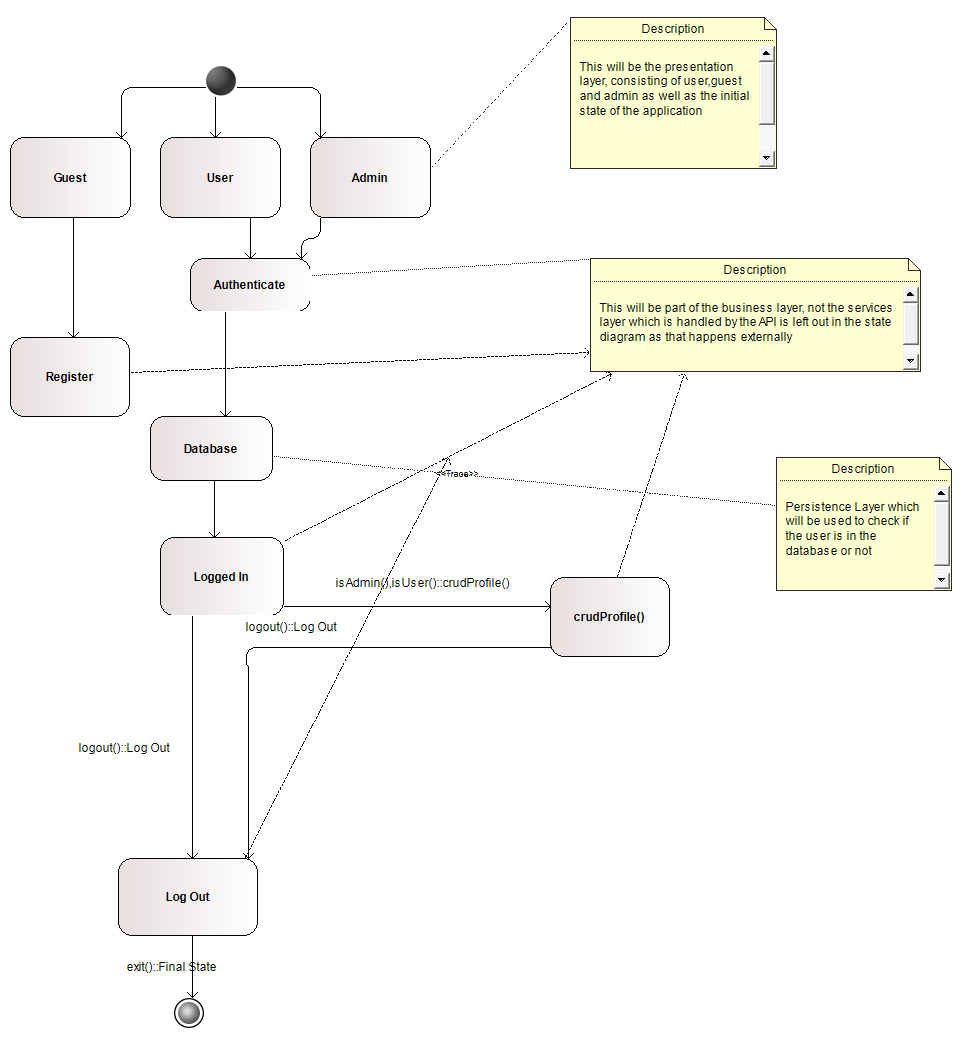
\includegraphics[scale=0.45]{smdu.png}
			
 		\end{itemize}
	\subsection{Technologies}
			\begin{itemize}
 				\item Presentation Layer
				\\
				\\
				For the presentation layer we will use android studio as well as iOS and Web front end. This is to make the application available on multiple platforms which is important
 			
				
 			
				\item Business Layer
				\\
				\\
				For the business layer we will use Java Enterprise Editions' REST API, this is for improved scalability since the client and server are loosely coupled.
 				
			
				\item Persistence Layer
				\\
				\\
				For the Persistence layer we will use Java Persistence API(JPA), for accessing, managing and persisting data between data transfer objects. This allows us to focus more on the object model than the actual SQL, enables us to save time by generating/updating SQL queries and convert the results to our model classes.
	
				
				\item Database Layer
				\\
				\\
				For the Database layer we will use JDBC, which offers a natural java interface therby making it easier to work with SQL, this works well since our persistence layer is generating SQL queries for u, allowing us to manage and manipulate the database.
				
			
 		\end{itemize}
	
\end{document}